\section{Реализация шаблонного подхода}

Одной из целей данной работы было доказательство того, что принтер можно задавать с помощью шаблонов.
Самый простой способ доказать это --- предъявить такой принтер. Было принято решение реализовать принтер для модельного языка L, уже описанного в этом тексте.

Работа принтера разбивается на два этапа: подготовка шаблонов и непосредственно печать синтаксического дерева.

На подготовительном этапе из файла с шаблонами языковых конструкций языка L строится набор образцов. \textit{Образцом} назовем пару из текста шаблона и обобщенного синтаксического дерева шаблона. Дерево шаблона --- обобщенное, так как на месте некоторых узлов стоят специальные метки, которые хранят информацию об ограничениях на текстовое представление соответствующих узлов.

Во время основной фазы работы принтера дерево, которое необходимо непачатать, будет сравниваться с деревьями из образцов. В случае согласованности образца и дерева для печати будет использоваться текст образца, в который на места меток будут вставлены представления соответствующих поддеревьев.

\subsection{Шаблон}

Внутри шаблона используется специальный язык разметки. Символы «\lstinline{@-}» на позиции поддерева синтаксической конструкции означают, что для применения данного шаблона поддерево должно быть напечатано в одну строку. Семантика символов «\lstinline{@* N @*}» совпадает с семантикой «\lstinline{@-}» с точностью до того, что напечатанное поддерево должно занимать строку длины не более N. Символы «\lstinline{@| @|}» означают, что соответствующее поддерево может быть напечатано и на нескольких строках. Для выделения отдельных шаблонов используются строки \lstinline{t_start}, \lstinline{t_end}.

Рассмотрим пример шаблонов для конструкции \lstinline{write} (см. рис. \ref{fig:writeTmplt1} и \ref{fig:writeTmplt2}).
Эти шаблоны задают именно такое представление \lstinline{write}, которого мы добивались в обзоре принтер-библиотек.
Благодаря шаблонам, необходимый результат получается просто и наглядно.

\begin{figure}[h!]
	\begin{subfigure}[h]{0.45\textwidth}
		\lstinputlisting{codes/writeTmplt1.l}
		\caption{}
		\label{fig:writeTmplt1}
	\end{subfigure}
	\begin{subfigure}[h]{0.45\textwidth}
		\lstinputlisting{codes/writeTmplt2.l}
		\caption{}
		\label{fig:writeTmplt2}
	\end{subfigure}
	\caption{Шаблоны для конструкции \lstinline{write}}
\end{figure}

Изначально в языке разметки не было конструкции «\lstinline{@* N @*}». Она кажется несколько неестественной. Действительно, при описаниях принтеров из введения и обзора ни разу не упоминалось, что нужно ограничение, которое не просто проверяет раскладку поддерева на однострочность.
Появление данной конструкции было вызвано тем, что многие поддеревья раскладовались в одну строчку. Получались слишком длинные строки. Рассмотрим случай вложенных операторов \lstinline{if-then-else}. Зададим шаблоны для печати оператора \lstinline{if-then-else} только с помощью «\lstinline{@-}» и «\lstinline{@| @|}» (см. рис. \ref{fig:flatBadIfTmplt} и \ref{fig:multBadIfTmplt}).

\begin{figure}[h!]
	\begin{subfigure}[h]{0.45\textwidth}
		\lstinputlisting{codes/flatBadIfTmplt.l}
		\caption{Однострочный вариант}
		\label{fig:flatBadIfTmplt}
	\end{subfigure}
	\begin{subfigure}[h]{0.45\textwidth}
		\lstinputlisting{codes/multBadIfTmplt.l}
		\caption{Многострочный вариант}
		\label{fig:multBadIfTmplt}
	\end{subfigure}
	\caption{Шаблоны для конструкции \lstinline{if-then-else}}
\end{figure}

Тогда дерево с вложенными \lstinline{if-then-else} будет представлено однострочно (см. рис. \ref{fig:nestedIf} и \ref{fig:nestedIfFlatCode}), чего хотелось бы избежать.

\begin{figure}[h!]
	\centering
	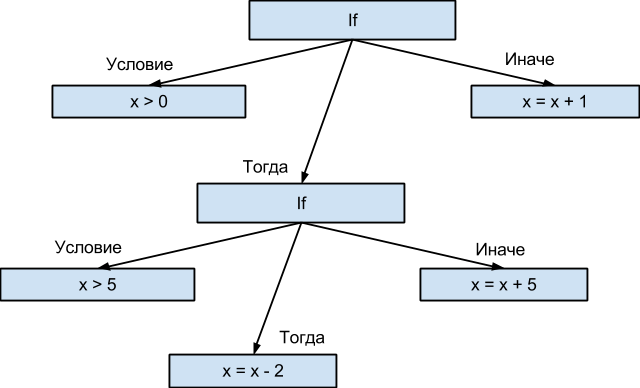
\includegraphics[width=0.6\textwidth]{nestedIf}
	\caption{Пример дерева вложенных \lstinline{if-then-else}}
	\label{fig:nestedIf}
\end{figure}

\begin{figure}[h!]
	\centering
	\lstinputlisting{codes/nestedIf.l}
	\caption{Представление с помощью шаблона с рис. \ref{fig:flatBadIfTmplt}}
	\label{fig:nestedIfFlatCode}
\end{figure}

Но если воспользоваться «\lstinline{@* N @*}», то можно переписать однострочный шаблон так, что подобная проблема не возникала (см. рис. \ref{fig:flatGoodIfTmplt} и \ref{fig:nestedIfCode}). В подобных ситуациях однострочный вариант просто не будет выбираться.

\begin{figure}[h!]
	\lstinputlisting{codes/flatGoodIfTmplt.l}
	\caption{Новый однострочный вариант шаблона для конструкции \lstinline{if-then-else}}
	\label{fig:flatGoodIfTmplt}	
\end{figure}

\begin{figure}[h!]
	\centering
	\lstinputlisting{codes/goodNestedIf.l}
	\caption{Представление с помощью новых шаблонов}
	\label{fig:nestedIfCode}
\end{figure}

Также одним из неочевидных свойств шаблонов является то, что с их помощью можно выражать не только базовые конструкции языка. Никто не мешает завести отдельный шаблон, описывающий ситуацию, к примеру, тех же вложенных \lstinline{if-then-else}. Но 

\subsection{Построение образцов}

Шаблоны могут быть использованы только в том случае, если мы можем сравнивать их синтаксическое представление с деревом, которое печатаем. Поэтому нам нужен синтаксический анализатор, понимающий язык разметки внутри языка L. То есть если исходный анализатор имеет тип \lstinline[language=Haskell]{parser :: String -> Statement}, то нужный анализатор должен иметь тип \lstinline[language=Haskell]{extendedParser :: String -> ExtendedStatement}, где тип \lstinline[language=Haskell]{ExtendedStatement} является расширением типа \lstinline[language=Haskell]{Statement} с отдельными конструкторами для меток из шаблонов. Кроме того, в конструкторах меток будет храниться информация о положении метки внутри строкового представления шаблона, чтобы на этапе печати документа знать, куда вставлять представления поддеревьев.

В результате работы расширенного анализатора получается набор образцов.

% Для получения такого анализатора возьмем анализатор языка L (см. рис. \ref{fig:lStmtParser}).

% \begin{figure}[h]
% 	\lstinputlisting[language=Caml]{codes/lStmtParser.ml}
% 	\caption{Синтаксический анализатор языка L}
% 	\label{fig:lStmtParser}
% \end{figure}

% \begin{figure}[h]
% 	\lstinputlisting[language=Caml]{codes/lExprParser.ml}
% 	\caption{Синтаксический анализатор языка L}
% 	\label{fig:lExprParser}
% \end{figure}

% Синтаксический анализатор языка L был обобщен с помощью анализатора, который разбирает рассмотренные конструкции. Таким образом, был получен расширенный анализатор, конструирующий по шаблонам набор обобщенных синтаксических деревьев, которые в дальнейшем используются при печати обычных синтаксических деревьев программ языка L.

\subsection{Сопоставление дерева с набором образцов}

TODO

% Для доказательства состоятельности подхода задания принтера с помощью шаблонов было принято решение разработать шаблонный принтер для модельного языка L.
% Работа принтера должна была выглядеть следующим образом:

% Сначала расширенный синтаксический анализатор языка L строит образцы 

% В ходе данной работы для доказательства состоятельности подхода построения принтера по набору шаблонных конструкций был выбран конструктивный способ.
% Для этого был реализован соответсвующий принтер для языка L.

% Работа над принтером состояла из нескольких частей:
% \begin{enumerate}
% 	\item разработка языка шаблонов;
% 	\item расширение синтасического анализатора языка L, чтобы он мог разбирать шаблонные выражения;
% 	\item реализация механизма принтера по имеющимся образцам
% 	(то есть сопоставление синтаксического дерева программы, которую нужно напечатать, с набором шаблонов).
% \end{enumerate}

% \subsection{Язык шаблонов}

% Шаблоны для языковым конструкций будем строить по подобию данной

% Обзор существующих библиотек и опыт написания принтеров показали, что основными конструкц